\begin{example} \label{Ex:3.2.Eg5}
Sketch $\ds f(x) = \frac{x^2-x-2}{x^2-x-6}$.

\solution We follow the steps outlined in the Curve Sketching Concept.

\begin{enumerate}[1)]
\item In determining the domain, we assume it is all real numbers and looks for restrictions. We find that at $x=-2$ and $x=3$, $f(x)$ is not defined. So the domain of $f$ is $D = \{\text{real numbers } x\ | \ x\neq -2,3\}$.

\item To find the critical values of $f$, we first find $f'(x)$. Using the Quotient Rule, we find 
$$f'(x) = \frac{-8x+4}{(x^2+x-6)^2} = \frac{-8x+4}{(x-3)^2(x+2)^2}.$$
		
We find that $\fp(x) = 0$ when $x = 1/2$, and $\fp$ is undefined when $x=-2,3$. 
		
\item To find the possible points of inflection, we find $\fpp(x)$, again employing the Quotient Rule: 
$$\fpp(x) = \frac{24x^2-24x+56}{(x-3)^3(x+2)^3}.$$
		
We find that $\fpp(x)$ is never $0$ (setting the numerator equal to $0$ and solving for $x$, we find the only roots to this quadratic are complex) and $\fpp$ is undefined when $x=-2,3$. Thus concavity will possibly only change at $x=-2$ and $x=3$.
		
\item The vertical asymptotes of $f$ are at $x=-2$ and $x=3$, the places where $f$ is undefined.
		
\item There is a horizontal asymptote of $y=1$, as $\ds \lim_{x\to -\infty}f(x) = 1$ and $\ds\lim_{x\to\infty}f(x) =1$.
		
\item We place the values $x=1/2$, $x=-2$ and $x=3$ on a number line as shown below. We mark in each interval whether $f$ is increasing or decreasing, concave up or down. We see that $f$ has a relative maximum at $x=1/2$; concavity changes only at the vertical asymptotes.

\begin{center}
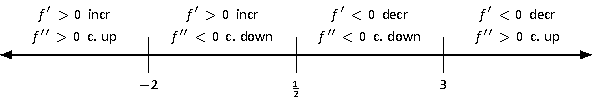
\includegraphics[scale=.75]{figures/figsketchline2}
\end{center}

\item In Figure~\ref{fig:sketch2}-(a), we plot the points from the number line on a set of axes and connect the points with straight lines to get a general idea of what the function looks like (these lines effectively only convey increasing/decreasing information). 

In Figure~\ref{fig:sketch2}-(b), we adjust the graph with the appropriate concavity. We also show $f$ crossing the $x$ axis at $x=-1$ and $x=2$.

Figure~\ref{fig:sketch2}-(c) shows a computer generated graph of $f$, which verifies the accuracy of our sketch.
\end{enumerate}
\end{example}

\begin{marginfigure}[-16cm] % MARGIN FIGURE
%\captionsetup[subfigure]{labelformat=empty}
\subfloat[]{\margingraphics{figures/figsketch2a}}

\subfloat[]{\margingraphics{figures/figsketch2b}}

\subfloat[]{\margingraphics{figures/figsketch2}}
\caption{Sketching $f$ in Example~\ref{Ex:3.2.Eg5}.}
\label{fig:sketch2}
\end{marginfigure}